\documentclass{beamer}
\usepackage{pgfplots}
\usepackage{tikz}
\usepackage{csquotes}
\usepackage{cancel}
\usetheme{metropolis}
\title{Resource Buying Games}
\author[C. Welzel]{Christoph Welzel}

\newcommand{\tupel}[1]{\left(#1\right)}
\newcommand{\set}[1]{\left\{#1\right\}}

\begin{document}
\definecolor{p1}{rgb}{1,0,0}
\definecolor{p2}{rgb}{0,0,1}
\definecolor{both}{rgb}{0.5,0,0.5}
\usetikzlibrary{arrows, cd, positioning, backgrounds, fit}
\tikzset{%
  node/.style={circle, inner sep=1pt, text width=0pt, text height=0pt, fill=black!100},
  edge/.style={thick, draw}
}
  

\maketitle
\section{Introduction}
\begin{frame}
\end{frame}

\subsection{Game definition}
\begin{frame}
  \frametitle{Definition: congestion model}
  \begin{equation*}
    \mathcal{M} = \tupel{N, E, \mathcal{S}, \left(d_{i}\right)_{i\in N},
    \left(c_{e}\right)_{e\in E}}
  \end{equation*}
  \vspace{-1cm}
  \begin{itemize}
    \item $N$: set of players
    \item $E$: set of resources
    \item $\mathcal{S} = \times_{i\in N}\mathcal{S}_{i}$ with $\mathcal{S}_{i}$
      set of desired resources $S_{i}\subseteq E$: set of configurations
    \item $d_{i}$: demand of player $i$ for her resource
      \begin{itemize}
        \item $d_{i} = 1$ for an unweighted game
        \item $\ell_{e}(S) = \sum_{i\in N:e\in S_{i}}d_{i}$: load of $e$
          in configuration $S\in\mathcal{S}$
      \end{itemize}
    \item $c_{e}:\mathbb{N}\rightarrow\mathbb{N}$ with
      $c_{e}(S) = c_{e}(\ell_{e}(S))$: cost for the resource $e$ under the load
      of $S$
  \end{itemize}
\end{frame}

\begin{frame}
  \frametitle{Definition: weighted resource buying game}
  \begin{equation*}
    \mathcal{M} = \tupel{N, E, \mathcal{S}, \left(d_{i}\right)_{i\in N},
    \left(c_{e}\right)_{e\in E}}
  \end{equation*}
  \begin{equation*}
    \leadsto\mathcal{G} = \tupel{N, \mathcal{S}\times\mathcal{P}, \pi}
  \end{equation*}
  \vspace{-1cm}
  \begin{itemize}
    \item $\mathcal{P}=\times_{i\in N} P_{i}$ with
      $P_{i} = \mathbb{R}^{|E|}_{+}$: payment of player $i$
    \item $e\in E$ is bought under $S\in \mathcal{S}$ if
      $\sum_{i\in N}p_{i}^{e} \geq c_{e}(S)$
    \item $\pi_{i}(S) =
      \begin{cases}
        \sum_{e\in E}p_{i}^{e} &\textit{if }S_{i}\textit{ is bought}\\
        \infty &\textit{otherwise}
      \end{cases}$: {private cost of player $i$}
  \end{itemize}
\end{frame}

\begin{frame}
  \frametitle{A few simplifications}
  \begin{itemize}
    \item \emph{unweighted} games
    \item marginally non-increasing cost-function $c_{e}$:
      \begin{equation*}
        c_{e}(x + \delta) - c_{e}(x) \geq c_{e}(y + \delta) - c_{e}(y)
        \;\;x\leq y, \delta \in \mathbb{N}
      \end{equation*}
      \begin{center}
        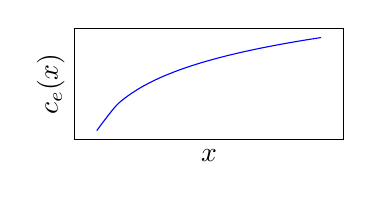
\begin{tikzpicture}
          \begin{axis}[
              xlabel=$x$,
              ylabel=$c_{e}(x)$,
              smooth,
              width=5cm,
              height=3cm,
              ticks=none,
              no markers
            ]
              \addplot{ln(x)};
          \end{axis}
        \end{tikzpicture}
      \end{center}
    \item restrict players demands to a specific mathematical structure:
      Matroids
  \end{itemize}
\end{frame}

\begin{frame}
  \frametitle{Definition: Matroid}
  \begin{columns}
    \column{0.5\textwidth}
    \begin{equation*}
      M = (E, B)
    \end{equation*}
    \vspace{-0.8cm}
    \begin{itemize}
      \item $E$: ground-set
      \item $B$: set of bases
      \item \emph{basis exchange property}:
        \vspace{-1cm}
        \begin{center}
          \begin{align*}
            \forall &X, Y\in B:\\
            &\forall x\in (X\setminus Y)\\
            &\exists y\in (Y\setminus X):\\
            &\;(X\setminus \set{x})\cup\{y\}\in B
          \end{align*}
        \end{center}
    \end{itemize}
    \column{0.5\textwidth}
    \uncover<2->{Spanning trees:}
    \begin{center}
      \uncover<2->{\resizebox{0.8\textwidth}{!}{\input{tikz/graphp1}}\\[0.5cm]}
      \uncover<3->{\resizebox{0.4\textwidth}{!}{\input{tikz/graphp1S1}}}
      \uncover<4->{\resizebox{0.4\textwidth}{!}{\begin{tikzpicture}
  \node[node] (A) {};
  \node[below=0.5 of A] (d1) {};
  \node[node, below=0.5 of d1] (B) {};
  \node[right=1 of A] (d2) {};
  \node[node, right=1 of d2] (D) {};
  \node[node] (C) at (d1-|d2) {};
  \node[node] (E) at (B-|D) {};

  \draw[edge, p1] (A) to (B);
  \draw[edge, p1, dotted] (A) to (C);
  \draw[edge, p1] (B) to (C);
  \draw[edge, p1] (C) to (D);
  \draw[edge, p1] (C) to (E);
\end{tikzpicture}
}}
      \uncover<5->{\resizebox{0.4\textwidth}{!}{\input{tikz/graphp1S3}}}
    \end{center}
  \end{columns}
\end{frame}

\begin{frame}
  \frametitle{Operations on Matroids $\mathcal{M} = \tupel{E, \mathcal{B}}$}
  \begin{columns}
    \column{0.5\textwidth}
    \begin{center}
      Contraction:
    \end{center}
    \vspace{-0.6cm}
    \begin{align*}
      &\mathcal{M}/e = \tupel{E\setminus\set{e}, \mathcal{B}/e}\text{ with}\\
      &\mathcal{B}/e = \set{B\subseteq (E\setminus\set{e})\middle| B\cup\set{e}\in\mathcal{B}}
    \end{align*}
    \column<4->{0.5\textwidth}
    \begin{center}
      Deletion:
    \end{center}
    \vspace{-0.6cm}
    \begin{align*}
      &\mathcal{M}\setminus e = \tupel{E\setminus\set{e},\mathcal{B}\setminus e}\text{ with}\\
      &\mathcal{B}\setminus e = \set{B\subseteq E\setminus\set{e}\middle|B\in\mathcal{B}}
    \end{align*}
  \end{columns}
  \begin{center}
    \begin{tikzpicture}
      \uncover<2->{\node (G) {\input{tikz/graphp1}};
      \node[right=1 of G] (leadsto) {\Huge$\leadsto$};}
      \uncover<3>{\node[right=1 of leadsto] (G') {\input{tikz/graphp1Cont}};}
      \uncover<5>{\node[right=1 of leadsto] (G'') {\begin{tikzpicture}
  \node[node] (A) {};
  \node[below=0.5 of A] (d1) {};
  \node[node, below=0.5 of d1] (B) {};
  \node[right=1 of A] (d2) {};
  \node[node, right=1 of d2] (D) {};
  \node[node] (C) at (d1-|d2) {};
  \node[node] (E) at (B-|D) {};

  \node[above left =0.1 and 0.1 of d1] (del1) {};
  \node[above right=0.1 and 0.1 of d1] (del2) {};
  \node[below left =0.1 and 0.1 of d1] (del3) {};
  \node[below right=0.1 and 0.1 of d1] (del4) {};

  \draw[edge, p1, dotted] (A) to (B);
  \draw[edge, p1] (A) to (C);
  \draw[edge, p1] (B) to (C);
  \draw[edge, p1] (C) to (D);
  \draw[edge, p1] (C) to (E);

  \draw[thick, black] (del1) to (del4);
  \draw[thick, black] (del2) to (del3);
\end{tikzpicture}
};}
    \end{tikzpicture}
  \end{center}
\end{frame}

\begin{frame}
  \frametitle{Cuts in Matroids}
  \begin{columns}
    \column{0.7\textwidth}
    $\mathcal{M} = \tupel{E, \mathcal{B}}$
    \begin{itemize}
      \item \emph{Cut}: inclusion-wise minimal $C\subseteq E$ such that
        $E\setminus C$ does not contain a basis of $\mathcal{M}$
      \item[$\leadsto$] $\mathcal{C}\tupel{\mathcal{M}} =
        \set{C\subseteq E\middle| C\text{ is a cut in } \mathcal{M}}$
    \end{itemize}
    \column{0.3\textwidth}
    \resizebox{0.8\textwidth}{!}{\input{tikz/graphp1}}
  \end{columns}
  \vspace{0.7cm}
  \begin{columns}
    \column{0.33\textwidth}
    \uncover<2->{\resizebox{0.7\textwidth}{!}{\input{tikz/graphp1Cut1}}\\[0.3cm]}
    \uncover<3->{\resizebox{0.7\textwidth}{!}{\input{tikz/graphp1Cut2}}}
    \column{0.33\textwidth}
    \uncover<4->{\resizebox{0.7\textwidth}{!}{\begin{tikzpicture}
  \node[node] (A) {};
  \node[below=0.5 of A] (d1) {};
  \node[node, below=0.5 of d1] (B) {};
  \node[right=1 of A] (d2) {};
  \node[node, right=1 of d2] (D) {};
  \node[node] (C) at (d1-|d2) {};
  \node[node] (E) at (B-|D) {};

  \draw[edge, p1] (A) to (B);
  \draw[edge, p1] (A) to (C);
  \draw[edge, p1, dotted] (B) to (C);
  \draw[edge, p1, dotted] (C) to (D);
  \draw[edge, p1, dotted] (C) to (E);
\end{tikzpicture}
}}\\[0.3cm]
    \uncover<5->{\resizebox{0.7\textwidth}{!}{\input{tikz/graphp1Cut4}}}
    \column{0.33\textwidth}
    \uncover<6->{\resizebox{0.7\textwidth}{!}{\input{tikz/graphp1Cut5}}}
  \end{columns}
\end{frame}

\section{Algorithm: PNE in Unweighted Matroid Games}
\subsection{Algorithm}
\begin{frame}
  \frametitle{Algorithm}
  \begin{tabular}{|lll|}
    \hline
    (i) & Init: &\hspace{-0.6cm}\parbox{0.8\textwidth}{
        \begin{itemize}
          \item \parbox{0.7\textwidth}{every player: empty working basis, complete ground-set, complete set of valid result bases}
          \item every resource: cost for next load, current load
        \end{itemize}
      }\\\hline
    (ii) & Find: &\hspace{-0.6cm}\parbox{0.8\textwidth}{
        \begin{itemize}
          \item inclusion-min (necessary cost)-max cut $C$
          \item minimal cost resource $e$ in $C$
          \item owner $i$ of $C$
        \end{itemize}
      }\\\hline
    (iii) & Pick: &\hspace{-0.6cm}\parbox{0.8\textwidth}{
        \begin{itemize}
          \item $i$: add $e$ to working basis, contract matroid to $e$
          \item $e$: update marginal cost and increase load
          \item all player: delete elements $C\setminus\set{e}$ from matroid
        \end{itemize}
      }\\\hline
    (iv) & Break: &\hspace{-0.6cm}\parbox{0.8\textwidth}{
        \begin{itemize}
          \item exists player with incomplete basis: goto (ii)
          \item otherwise: return chosen bases and payments
        \end{itemize}
      }\\\hline
  \end{tabular}
\end{frame}

\begin{frame}
  \frametitle{Example: Graph}
  \begin{columns}
    \column{0.5\textwidth}
    Player 1:\\
    \vspace{-0.2cm}
    \begin{center}
      \resizebox{0.6\textwidth}{!}{\begin{tikzpicture}
  \node[node, label=$A$] (A) {};
  \node[below=0.5 of A] (d1) {};
  \node[node, below=0.5 of d1] (B) {};
  \node[right=1 of A] (d2) {};
  \node[node, right=1 of d2, label=$D$] (D) {};
  \node[node, label=$C$] (C) at (d1-|d2) {};
  \node[node] (E) at (B-|D) {};

  \draw[edge, p1] (A) to (B);
  \draw[edge, p1] (A) to (C);
  \draw[edge, p1] (B) to (C);
  \draw[edge, p1] (C) to (D);
  \draw[edge, p1] (C) to (E);
\end{tikzpicture}
}
    \end{center}
    \column{0.5\textwidth}
    Player 2:\\
    \vspace{-0.5cm}
    \begin{center}
      \resizebox{0.6\textwidth}{!}{\begin{tikzpicture}
  \node[node, label=$A$] (A) {};
  \node[below=0.5 of A] (d1) {};
  \node[right=1 of A] (d2) {};
  \node[node, right=1 of d2, label=$D$] (D) {};
  \node[node, label=$C$] (C) at (d1-|d2) {};
  \node[node, above=0.5 of d2] (F) {};

  \draw[edge, p2] (A) to (C);
  \draw[edge, p2] (C) to (D);
  \draw[edge, p2] (A) to (F);
  \draw[edge, p2] (D) to (F);
\end{tikzpicture}
}
    \end{center}
  \end{columns}
  \begin{center}
    \resizebox{0.35\textwidth}{!}{\begin{tikzpicture}
  \node[node] (A) {};
  \node[below=0.5 of A] (d1) {};
  \node[node, below=0.5 of d1] (B) {};
  \node[right=1 of A] (d2) {};
  \node[node, right=1 of d2] (D) {};
  \node[node] (C) at (d1-|d2) {};
  \node[node] (E) at (B-|D) {};
  \node[node, above=0.5 of d2] (F) {};

  \draw[edge, p1] (A) to (B);
  \draw[edge, both] (A) to (C);
  \draw[edge, p1] (B) to (C);
  \draw[edge, both] (C) to (D);
  \draw[edge, p1] (C) to (E);
  \draw[edge, p2] (A) to (F);
  \draw[edge, p2] (D) to (F);
\end{tikzpicture}
}
  \end{center}
\end{frame}

\newlength{\cutscaling}
\setlength{\cutscaling}{0.17\textwidth}
\begin{frame}
  \frametitle{Example: Algorithm}
  \begin{columns}
    % left column:
    \column{0.3\textwidth}
    \resizebox{\textwidth}{!}{\alt<1-6>{\input{tikz/graphp1}}{\alt<7>{\input{tikz/graphp1Cont}}{\begin{tikzpicture}
  \node[node] (A) {};
  \node[below=0.5 of A] (d1) {};
  \node[node, below=0.5 of d1] (B) {};
  \node[right=1 of A] (d2) {};
  \node[node, right=1 of d2] (D) {};
  \node[node] (C) at (d1-|d2) {};
  \node[node] (E) at (B-|D) {};
  
  \node[fit=(A) (B), draw, rectangle, rounded corners, black] (new) {};

  \draw[edge, p1, bend right, dotted] (C) to (new.east);
  \draw[edge, p1, bend left] (C) to (new.east);
  \draw[edge, p1] (A) to (B);
  \draw[edge, p1] (C) to (D);
  \draw[edge, p1] (C) to (E);
\end{tikzpicture}
}}}
    \begin{columns}
      \column{0.5\textwidth}
      \resizebox{\cutscaling}{!}{\alt<1-2>{\input{tikz/graphp1Cut1}}{\input{tikz/graphp1Cut1value}}}
      \resizebox{\cutscaling}{!}{\alt<1-3>{\input{tikz/graphp1Cut2}}{\input{tikz/graphp1Cut2value}}}
      \resizebox{\cutscaling}{!}{\alt<1-3>{\begin{tikzpicture}
  \node[node] (A) {};
  \node[below=0.5 of A] (d1) {};
  \node[node, below=0.5 of d1] (B) {};
  \node[right=1 of A] (d2) {};
  \node[node, right=1 of d2] (D) {};
  \node[node] (C) at (d1-|d2) {};
  \node[node] (E) at (B-|D) {};

  \draw[edge, p1] (A) to (B);
  \draw[edge, p1] (A) to (C);
  \draw[edge, p1, dotted] (B) to (C);
  \draw[edge, p1, dotted] (C) to (D);
  \draw[edge, p1, dotted] (C) to (E);
\end{tikzpicture}
}{\input{tikz/graphp1Cut3value}}}
      \column{0.5\textwidth}
      \resizebox{\cutscaling}{!}{\alt<1-3>{\input{tikz/graphp1Cut4}}{\input{tikz/graphp1Cut4value}}}
      \resizebox{\cutscaling}{!}{\alt<1-3>{\input{tikz/graphp1Cut5}}{\input{tikz/graphp1Cut5value}}}
    \end{columns}

    % middle column:
    \column{0.4\textwidth}
    \resizebox{\textwidth}{!}{\alt<1-8>{\input{tikz/graphbothCosts}}{\begin{tikzpicture}
  \node[node] (A) {};
  \node[below=0.5 of A] (d1) {};
  \node[node, below=0.5 of d1] (B) {};
  \node[right=1 of A] (d2) {};
  \node[node, right=1 of d2] (D) {};
  \node[node] (C) at (d1-|d2) {};
  \node[node] (E) at (B-|D) {};
  \node[node, above=0.5 of d2] (F) {};

  \draw[edge, p1] (A) to node[right, black, label={[black,label distance=-0.2cm]right:\tiny$8$}] {\tiny\bcancel{$7$}} (B);
  \draw[edge, both, dotted] (A) to node[above, black] {\tiny$8$} (C);
  \draw[edge, p1] (B) to node[below, black] {\tiny$2$} (C);
  \draw[edge, both] (C) to node[above, black] {\tiny$3$} (D);
  \draw[edge, p1] (C) to node[below, black] {\tiny$6$} (E);
  \draw[edge, p2] (A) to node[above, black] {\tiny$5$} (F);
  \draw[edge, p2] (D) to node[above, black] {\tiny$2$} (F);
\end{tikzpicture}
}}
    \begin{center}
      \uncover<5->{\alt<5>{\resizebox{0.7\textwidth}{!}{\begin{tikzpicture}
  \node[node] (A) {};
  \node[below=0.5 of A] (d1) {};
  \node[node, below=0.5 of d1] (B) {};
  \node[right=1 of A] (d2) {};
  \node[node, right=1 of d2] (D) {};
  \node[node] (C) at (d1-|d2) {};
  \node[node] (E) at (B-|D) {};

  \draw[edge, p1] (A) to (B);
  \draw[edge, p1] (A) to (C);
  \draw[edge, p1, dotted] (B) to (C);
  \draw[edge, p1, dotted] (C) to (D);
  \draw[edge, p1, dotted] (C) to (E);
\end{tikzpicture}
}}{\resizebox{0.7\textwidth}{!}{\input{tikz/graphp1Cut3marked}}}}
    \end{center}

    % right column:
    \column{0.3\textwidth}
    \resizebox{\textwidth}{!}{\alt<1-7>{\begin{tikzpicture}
  \node[node] (A) {};
  \node[right=1 of A] (d1) {};
  \node[node, right=1 of d1] (C) {};
  \node[above=0.5 of C] (d2) {};
  \node[node] (B) at (d2-|d1) {};
  \node[node, above=0.5 of d2] (D) {};
  \node[node, above=0.2 of D] (E) {};

  \draw[edge, p2] (A) to (B);
  \draw[edge, p2] (B) to (D);
  \draw[edge, p2] (C) to (D);
  \draw[edge, p2] (B) to (E);
  \draw[edge, p2, bend right] (C) to (E);
\end{tikzpicture}
}{\input{tikz/graphp2Del}}}
    \begin{columns}
      \column{0.5\textwidth}
      \resizebox{\cutscaling}{!}{\alt<1-3>{\input{tikz/graphp2Cut1}}{\input{tikz/graphp2Cut1value}}}
      \resizebox{\cutscaling}{!}{\alt<1-3>{\begin{tikzpicture}
  \node[node] (A) {};
  \node[below=0.5 of A] (d1) {};
  \node[right=1 of A] (d2) {};
  \node[node, right=1 of d2] (D) {};
  \node[node] (C) at (d1-|d2) {};
  \node[node, above=0.5 of d2] (F) {};

  \draw[edge, p2] (A) to (C);
  \draw[edge, p2, dotted] (C) to (D);
  \draw[edge, p2, dotted] (A) to (F);
  \draw[edge, p2] (D) to (F);
\end{tikzpicture}
}{\input{tikz/graphp2Cut2value}}}
      \resizebox{\cutscaling}{!}{\alt<1>{\input{tikz/graphp2Cut3}}{\input{tikz/graphp2Cut3deleted}}}
      \column{0.5\textwidth}
      \resizebox{\cutscaling}{!}{\alt<1>{\input{tikz/graphp2Cut4}}{\begin{tikzpicture}
  \node[node] (A) {};
  \node[below=0.5 of A] (d1) {};
  \node[right=1 of A] (d2) {};
  \node[node, right=1 of d2] (D) {};
  \node[node] (C) at (d1-|d2) {};
  \node[node, above=0.5 of d2] (F) {};

  \node[above left=0.25 and 0.25 of d2] (cross0.5) {};
  \node[above right=0.25 and 0.25 of d2] (cross2) {};
  \node[below right=0.25 and 0.25 of d2] (cross3) {};
  \node[below left=0.25 and 0.25 of d2] (cross4) {};

  \draw[very thick, red] (cross1) to (cross3);
  \draw[very thick, red] (cross2) to (cross4);

  \draw[edge, p2, dotted] (A) to (C);
  \draw[edge, p2] (C) to (D);
  \draw[edge, p2] (A) to (F);
  \draw[edge, p2, dotted] (D) to (F);
\end{tikzpicture}
}}
      \resizebox{\cutscaling}{!}{\alt<1>{\input{tikz/graphp2Cut5}}{\input{tikz/graphp2Cut5deleted}}}
      \resizebox{\cutscaling}{!}{\alt<1-3>{\input{tikz/graphp2Cut6}}{\input{tikz/graphp2Cut6value}}}
    \end{columns}
  \end{columns}
  \uncover<9>{ }
\end{frame}

\begin{frame}
  \frametitle{Soundness}
  \begin{itemize}
    \item Termination:
      \begin{itemize}
        \item inductively applying contraction operations lead to basis
        \item deletion cannot \enquote{loose} bases for other players since
          chosen cut is inclusion-wise minimal
      \end{itemize}
    \item Correctness
      \begin{itemize}
        \item Lemma: cost of the chosen element decreases monotonically in each
          iteration
        \item assume there is a beneficial alternative basis
          $\hat{B} = (B_{i}\setminus\set{g})\cup{f}$
          \begin{itemize}
            \item consider iteration $k$ in which $g$ is added to basis of $i$:
            \item if $f$ is in the corresonponding cut its cost never changes
              since it is deleted from every matroid $rightarrow$ $f$ is not in
              the cut
            \item but $f$ and $g$ \enquote{open} same dimensionality, thus $f$
              is not left in contracted matroid of $i$
            \item $f$ was deleted before (in this iteration the cost of the
              chosen element was lower than for $f$ in contradiction to lemma)
          \end{itemize}
      \end{itemize}
  \end{itemize}
\end{frame}

\section{Weighted Matroid Games}
\begin{frame}
  % \begin{itemize}
  %   \item (2 slides)
  %   \item Introduce socially optimal solution
  %   \item Show (or at least motivate) why this is a PNE
  %   \item Mention reduction to show that finding an optimal solution is
  %     NP-hard
  % \end{itemize}
\end{frame}

\section{Non-Matroid Strategy Spaces}
\subsection{Lack of PNE}
\begin{frame}
  % \begin{itemize}
  %   \item (1 slide)
  %   \item Present that for Non-Matroid Games we can find strategy spaces
  %     which do not allow PNE
  %   \item Illustrate the construction by a picture
  % \end{itemize}
\end{frame}

\subsection{Non-Decreasing Marginal Cost Functions \& Price of Anarchy}
\begin{frame}
  % \begin{itemize}
  %   \item (3 slides)
  %   \item Present that games with Non-Decreasing Marginal Cost Functions allow
  %     PNE (explain how the marginal cost pricing is obtained)
  %   \item Define Price of Anarchy
  %   \item Mention that non-increasing and non-decreasing games with weighted
  %     players is unbounded
  % \end{itemize}
\end{frame}

\section{Conclusion}
\begin{frame}
  % \begin{itemize}
  %   \item (1 slide)
  %   \item Sum up results
  %   \item Embed results into topic
  % \end{itemize}
\end{frame}

\end{document}
